\chapter{Validation of Modified TASC Results with Experimental Data} \label{chap:experiment-validation-tasc}

The final demonstration of the modified TASC program for bending models is to validate its interpolation of bending results against a four-point bend experiment, similar to what was interpolated manually in \Cref{chap:experiment-validation}.
%After TASC has been modified, use it to validate.
Input data for TASC included
plate dimensions of \(W_\text{test}=3.00\)~inch and \(t_\text{test}=0.374\)~inch,
roller span distances of \(S_\text{outer,test}=10.168\)~inch and \(S_\text{inner,test}=4.00\)~inch,
crack dimensions of \(a_\text{test}=0.215\)~inch, \(2c_\text{test}=0.490\)~inch,
and
material properties of \(E=10800\)~ksi, \(n=9\), and \(\Sys=56.0\)~ksi, as seen in \Cref{fig:tasc-force-cmod-validation}.
The modified TASC program calculated a predicted load-CMOD curve, and \Cref{fig:experimental-validation} shows the predicted curve compared to the actual test data.
The curves are within 2.6\% of each other at the end of the experimental range.
%Use \(\frac{a}{c}=0.878\), \(\frac{a}{t}=0.575\), \(\frac{E}{\Sys}=192.3\), \(n=9\), and \(\Sys=56.0\).
%Real specimen dimensions are \(W_\text{test}=3.00\)~inch and \(t_\text{test}=0.374\)~inch, crack dimensions of \(a_\text{test}=0.215\)~inch, \(2c_\text{test}=0.490\)~inch, and roller span distances of \(S_\text{outer,test}=10.168\)~inch and \(S_\text{inner,test}=4.00\)~inch.

\begin{figure}[tbp]
\centering
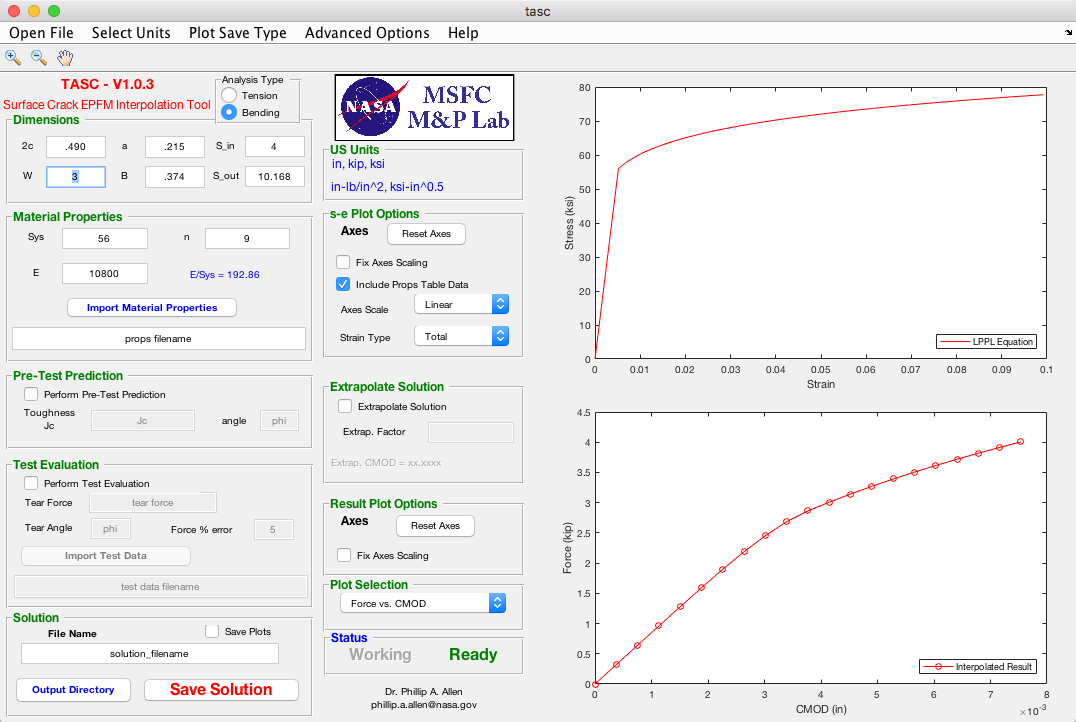
\includegraphics[width=0.8\columnwidth]{tasc-force-cmod-validation}
\caption{\label{fig:tasc-force-cmod-validation} Screenshot of TASC with parameters matching bend experiment}
\end{figure}

\begin{figure}[tbp]
\centering
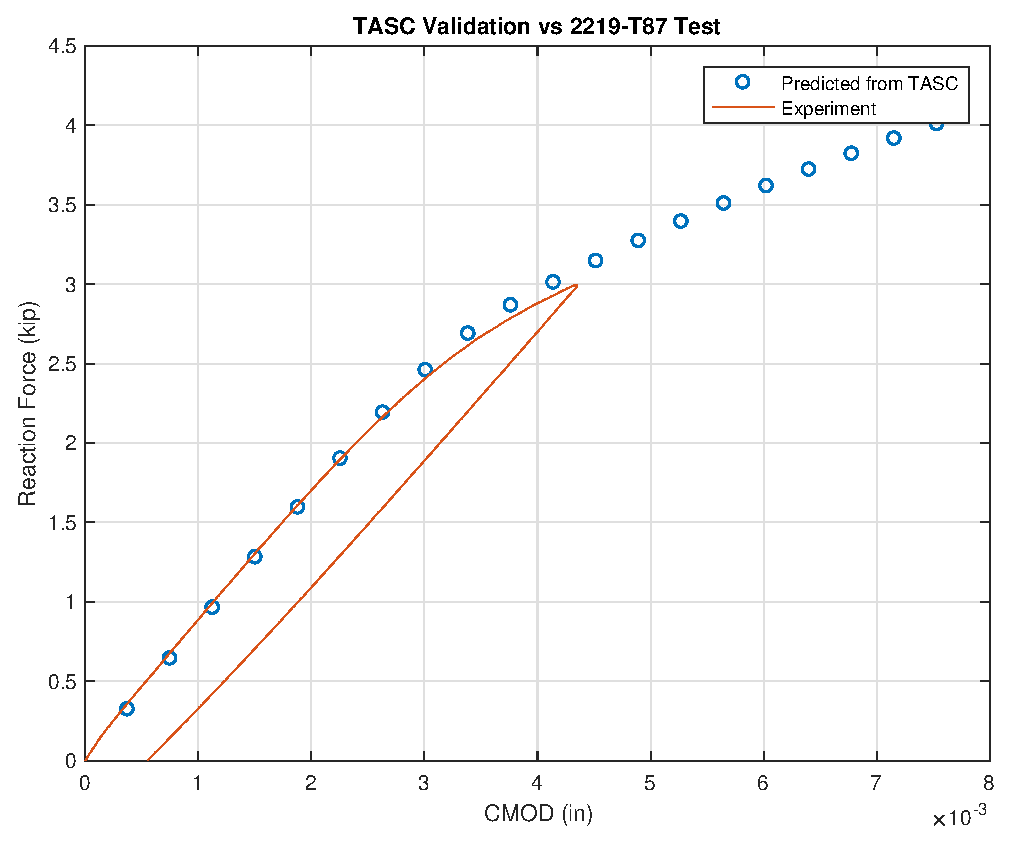
\includegraphics[width=0.8\columnwidth]{experimental-validation}
\caption{\label{fig:experimental-validation} Comparison of interpolated TASC model against bending experiment}
\end{figure}
